\chapter{Description et caractérisation de la matière à l'échelle macroscopique}

\intro{À notre échelle, la matière nous apparaît sous forme solide, liquide ou gazeuse.
 Elle est constituée d'une même espèce chimique ou peut être un mélange en apparence 
homogène ou hétérogène. Le chimiste ou le physicien va pouvoir analyser la composition
de la matière en pesant et mesurant des volumes de matière.}

%%%%%%%%%%%%%%%%%%%%%%%%%%%%%%%%%%%%%%%%%%%%%%%%%%%%%%%%%%%%%%%%%%%%%
\section{Corps purs et mélanges}

\subsection{Corps pur}
\paragraph{Définition} Un \textit{corps pur} est composé d'une seule espèce
chimique.
\paragraph{Exemple} L'eau distillée ne contient que des molécules d'eau
$H_2 O$, le cuivre pur ne contient que les atomes de $Cu$, le dioxygène
n'est constitué que de molécules $O_2$.

\subsection{Mélange} 
\paragraph{Définition} Un \textit{mélange contient plusieurs espèces chimiques}.
Le mélange est \textit{homogène} si les espèces chimiques ne sont
pas discernables. Dans le cas contraire, le mélange est \textit{hétérogène}.
\paragraph{Exemple} L'air, l'eau salée ou sucrée sont des mélanges homogènes.
Le sang, le lait sont des mélanges hétérogènes.


\subsection{Identification d'espèces chimiques par des méthodes physiques}
\paragraph{Méthodes physiques} Une \textit{espèce chimique} peut être identifiée 
par
\begin{itemize}
 \item ses températures de changement d'état
 \item sa masse volumique $ \rho$ par rapport à celle de l'eau 
\end{itemize}
La masse volumique de l'eau vaut $ \rho = 1.0~g.mL^{-1}$.

\paragraph{Masse volumique $\rho$} La \textit{masse volumique $\rho$} d'un corps (solide, liquide ou gaz) est le coefficient de proportionnalité entre sa masse $m$ et son volume $V$. 
$$ m = \rho \times V$$
L'unité de la masse volumique dépend des unités choisies pour la masse et le volume. Si $m$ est en gramme ($g$) et $V$ en millilitre ($mL$) alors $\rho$ est en gramme par millilitre ($g.mL^{-1}$).


\subsection{Identification d'espèces chimiques par des méthodes chimiques}
\paragraph{Test de présence de l'eau} 
La présence d'eau peut être mise en évidence par le test au sulfate de cuivre anhydre, poudre de
couleur blanche, qui devient bleue en présence d'eau. On peut verser une goutte de liquide à 
tester dessus ou déposer un peu de poudre sur un solide où on cherche la présence d'eau (figure 
\ref{fig:test_presence_eau}).
\begin{figure}[h]
  \begin{center}
      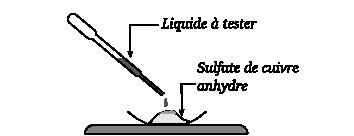
\includegraphics[width=\columnwidth]{1.1.-melanges/test_presence_eau.pdf}
  \end{center}
  \caption{La présence d'eau est confirmée par la coloration en bleu du sulfate de cuivre anhydre}
  \label{fig:test_presence_eau}
\end{figure}

\paragraph{Test de présence du dihydrogène}
Le dihydrogène $H_2$ se détecte par le test de la flamme qui provoque une petite explosion (figure 
\ref{fig:test_presence_H2}).
Attention, la quantité de gaz à tester doit être très faible, dans un petit tube à essai, 
car la réaction de combustion est très violente!
\begin{figure}[h]
  \begin{center}
      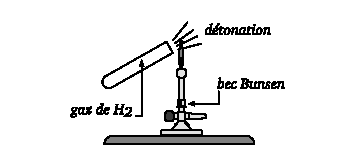
\includegraphics[width=\columnwidth]{1.1.-melanges/test_presence_H2.pdf}
  \end{center}
  \caption{La présence de dihydrogène est confirmée par une explosion. Attention, ce test doit être
  fait avec de très petites quantités de gaz, l'explosion étant très violente.}
  \label{fig:test_presence_H2}
\end{figure}

\paragraph{Test de présence du dioxygène}
Le dioxygène se détecte en plaçant un charbon incandescent dans un récipient où il y a du dioxygène.
Le charbon va s'enflammer grâce à l'oxygène (figure \ref{fig:test_presence_O2}).
\begin{figure}[h]
  \begin{center}
      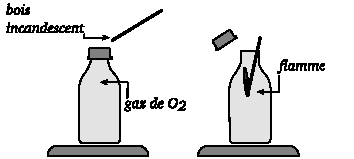
\includegraphics[width=\columnwidth]{1.1.-melanges/test_presence_O2.pdf}
  \end{center}
  \caption{La présence de dioxygène ravive une flamme à l'extrémité d'un bout de bois incandescent.}
  \label{fig:test_presence_O2}
\end{figure}

\paragraph{Test de présence du dioxyde de carbone}
Le dioxyde de carbone se détecte en faisant barboter le gaz dans de l'eau de chaux, qui va se troubler à
cause de la formation d'un précipité (figure \ref{fig:test_presence_CO2}).
\begin{figure}[h]
  \begin{center}
      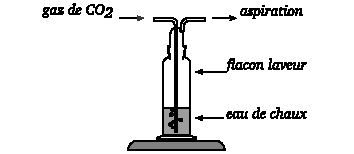
\includegraphics[width=\columnwidth]{1.1.-melanges/test_presence_CO2.pdf}
  \end{center}
  \caption{La présence de dioxyde de carbone trouble l'eau de chaux où barbote le gaz à tester.}
  \label{fig:test_presence_CO2}
\end{figure}


%%%%%%%%%%%%%%%%%%%%%%%%%%%%%%%%%%%%%%%%%%%%%%%%%%%%%%%%%%%%%%%%%%%%%
\section{Composition d'un mélange}
\subsection{Composition en masse}
\paragraph{Définition} Dans un \textit{mélange d'espèces chimiques} de masse totale $m$,
une des espèces chimiques a une masse $m_i$. On calcule alors son 
\textit{pourcentage en masse} grâce à la formule $$ \frac{m_i}{m} \times 100$$
qui s'exprime en $\%~mas $. Donner la \textit{composition en masse du mélange}
c'est donner les pourcentages en masse de tous les composants.
\paragraph{Exemples} Une solution contient $5.00~g$ d'hydroxyde de sodium $NaOH$
dans $100~g$ d'eau. La masse totale sera $m=100 + 5 = 105~g$ et donc le pourcentage
en masse d'hydroxyde sera $$\frac{5.00}{105} \times 100 = 4.77~\%~mas$$ \\
On veut savoir quelles masses de chlorure de sodium $NaCl$ et d'eau $H_{2}O$ prendre
pour avoir $175~g$ d'une solution à $15~\%~mas$ en chlorure de sodium. Si j'appelle
$a$ la masse de chlorure de sodium et $b$ la masse d'eau, je peux écrire que la masse
totale sera $$ a + b = 175~g$$ Si il y a $15~\%~mas$ en chlorure de sodium, je peux 
aussi écrire que $$ \frac{b}{175} \times 100 = 15$$ En divisant à gauche et à droite 
par $100$ puis en simplifiant $$ \frac{b}{175} = 0.15$$ et enfin en multipliant à 
gauche et à droite par $175$ et en simplifiant $$b = 26.25$$ c'est à dire qu'il faut
une masse de chlorure de sodium $b=26.25~g$ qu'on dissoudra dans une masse $a = 175 -b=
148.75~g$ d'eau.
\subsection{Composition en volume}
\paragraph{Définition}Dans un mélange d'espèces chimiques de volume total $V$, 
une des espèces chimiques a un volume $V_i$. On calcule alors son 
\textit{pourcentage en volume} grâce à la formule $$ \frac{V_i}{V} \times 100$$
qui s'exprime en $\%~vol $. Donner la \textit{composition en volume du mélange}
c'est donner les pourcentages en volume de tous les composants.
\paragraph{Cas de l'air} L'air que nous respirons a la composition en volume moyenne
suivante (tableau \ref{tab:composition_atmosphere}).
\begin{table}[h!]
  \centering
  \begin{tabu} to 0.95\linewidth {  X[2,l]  X[c]  }
    \hline
      \multirow{2}{4em}{\textbf{Élément}} & \textbf{Volume} \\
				      & \textbf{(en $\%~vol$)} \\
    \hline
      Azote $N_2$ & $78.09$ \\
      Oxygène $O_2$ & $20.95$ \\
      Argon $Ar$ & $0.93$ \\
      Dioxyde de carbone $CO_2$ & $0.035$ \\
      Autres gaz &  $...$ \\ 
    \hline
  \end{tabu}
  \caption{Composition en volume de l'atmosphère terrestre}
  \label{tab:composition_atmosphere}
\end{table}
\paragraph{Exemple} Si on prend un volume d'air $V=5.2~L$, alors
d'après le tableau \ref{tab:composition_atmosphere}, comme la 
composition en volume en azote est de $78.09~\%$, on peut écrire
$$ \frac{V_i}{5.2~L}\times 100 = 78.09$$ On divise à gauche et à droite 
par $100$ puis on multiplie à gauche et à droite par $5.2~L$, on
a alors le volume d'azote $$V_i = 4.1~L$$


%%%%%%%%%%%%%%%%%%%%%%%%%%%%%%%%%%%%%%%%%%%%%%%%%%%%%%%%%%%%%%%%%%%%%
\section{Solutions aqueuses}
\subsection{Solution}
\paragraph{Définition} Une \textit{solution} se constitue d'un liquide
\textit{le solvant} dans lequel est dissout \textit{le soluté} qui est
une espèce chimique moléculaire ou ionique. Voir la figure \ref{fig:solution}. Si le solvant est de l'eau,
on parle de \textit{solution aqueuse}.
\begin{figure}[h!]
  \begin{center}
      \includegraphics[width=0.8\columnwidth]{1.3.-schema-solution/schema_solution.pdf}
  \end{center}
  \caption{Une solution se compose d'un soluté dissout dans un solvant}
  \label{fig:solution}
\end{figure}


\subsection{Concentration en masse}
\paragraph{Définition} La \textit{concentration en masse $Cm$} d'une solution
est le rapport entre la masse $m$ de \textit{soluté} présent et le volume
$V$ de \textit{solution} $$Cm = \frac{m}{V}$$
Les unités sont
\begin{itemize}
 \item pour la masse $m$: le gramme $g$
 \item pour le volume $V$: le litre $L$
 \item pour la concentration en masse $Cm$: le gramme par litre $g.L^{-1}$
\end{itemize}

\subsection{Concentration maximale}
\paragraph{Définition} Pour un \textit{soluté donné}, il existe une 
\textit{concentration maximale} que l'on peut atteindre et au delà de laquelle
le \textit{soluté apporté} n'est plus capable de se dissoudre dans le solvant. Voir figure \ref{fig:solution_saturee}.
\begin{figure}[h!]
  \begin{center}
      \includegraphics[width=\columnwidth]{1.3.-schema-solution/solution_saturee.pdf}
  \end{center}
  \caption{Une solution de concentration en masse théorique $t$ supérieure à une concentration maximale $t_{max}$ ne sera 
  pas réalisable, car il restera du solide impossible à dissoudre car la concentration maximale est atteinte.}
  \label{fig:solution_saturee}
\end{figure}

\paragraph{Exemple}
On peut dissoudre au maximum $358~g$ de chlorure de sodium dans $1.00~L$ d'eau à $20~{}^o C$. 
Pour le chlorure d'argent, on peut dissoudre dans $1~L$ d'eau pur seulement $2,4~mg$ de ce sel.
Pour le glucose, on peut dissoudre dans un litre d'eau environ $900~g$ de cristaux de glucoses.

\subsection{Réalisation d'une solution} Pour fabriquer un volume $V$
de solution de \textit{concentration en masse} $Cm$, on doit peser une masse $m$
de soluté de manière à avoir une concentration en masse $$Cm=\frac{m}{V}$$
Ensuite, on procède à sa dissolution dans une fiole jaugée de volume $V$.
Voir figure \ref{fig:fab-sol-dissolution} page \pageref{fig:fab-sol-dissolution}.

\begin{figure*}[h!]
  \begin{center}
      \includegraphics[width=\textwidth]{1.3.-schema-solution/fab-sol-dissolution.pdf}
  \end{center}
  \caption{Fabrication d'une solution par dissolution}
  \label{fig:fab-sol-dissolution}
\end{figure*}


\subsection{Dilution d'une solution}
Si on a une \textit{solution mère} de concentration en masse $Cm_{\text{mère}}$
et de volume $V_\text{mère}$ on peut fabriquer une \textit{solution fille} de volume
$V_\text{fille}$ et de concentration $Cm_\text{fille}$ en ajoutant du solvant et on aura la relation $$ V_\text{fille} \times Cm_\text{fille} = V_\text{mère} \times Cm_\text{mère}$$
Voir figure \ref{fig:fab-sol-dilution} page \pageref{fig:fab-sol-dilution}.

\begin{figure*}[h!]
  \begin{center}
      \includegraphics[width=\textwidth]{1.3.-schema-solution/fab-sol-dilution.pdf}
  \end{center}
  \caption{Fabrication d'une solution par dilution.}
  \label{fig:fab-sol-dilution}
\end{figure*}


%%%%%%%%%%%%%%%%%%%%%%%%%%%%%%%%%%%%%%%%%%%%%%%%%%%%%%%%%%%%%%%%%%%%%
\section{Dosage par étalonnage}
\subsection{Dosage}
\paragraph{Définition}
Faire un \textit{dosage} en chimie, c'est \textit{mesurer la
concentration} d'une espèce chimique dans une solution. Pour mesurer 
cette concentration, on utilise des méthodes physiques ou chimiques.
\paragraph{Exemple} Les grandeurs que l'on peut utiliser pour mesurer
une concentration peuvent être la masse volumique, la couleur, la conductivité
électrique, le pH, etc. ...

\subsection{Étalonnage}
\paragraph{Définition}
Pour réaliser un \textit{dosage par étalonnage} d'une espèce chimique en solution, on \textit{fabrique
des solutions étalons} dont on connaît précisément la concentration et on mesure une grandeur
physique correspondant à cette solution. Ensuite, après avoir tracé une \textit{courbe 
d'étalonnage}, on mesure la même grandeur physique pour la solution inconnue et on en déduit 
la valeur de sa concentration \textit{par comparaison}.
\paragraph{Exemple}
Pour doser le saccharose dans $1~L$ de \textit{Coca Cola}, on a fabriqué par dissolution quatre solutions étalons de $100~mL$ de concentration en masse précise dont on mesure ensuite la masse volumique $\rho $. On trace   la masse volumique en fonction de la concentration en masse, puis après avoir mesuré la masse volumique du Coca Cola, on en déduit la concentration en masse en saccharose $t_{\textit{Coca Cola}} = 106~g.L^{-1}$.
Voir figure \ref{fig:courbe_etalonnage_cocacola}.
\begin{figure}[h!]
  \begin{center}
      \includegraphics[width=0.9\columnwidth]{1.3.-schema-solution/courbe_etalonnage_cocacola.pdf}
  \end{center}
  \caption{Dosage par étalonnage de la concentration en masse en saccharose du \textit{Coca Cola}.}
  \label{fig:courbe_etalonnage_cocacola}
\end{figure}

      